\section{Phase 4: Translating the AST to an EST}
\label{sec:astest}

This phase generates an Erlang syntax tree (EST) based on an AST. The purpose of this phase is to translate the abstract representation of a program into an Erlang program represented as a tree. The control flow, represented by goto statements in the AST, is translated into the functional language paradigm equivalent \emph{function calls}. Since functional languages are stateless the state is passed along in the function calls. Processes are native in the Erlang language, thus each process in the AST is simply translated into a module. The generated modules are spawned in a special \emph{system} module.

\begin{figure}[b!]
\centering
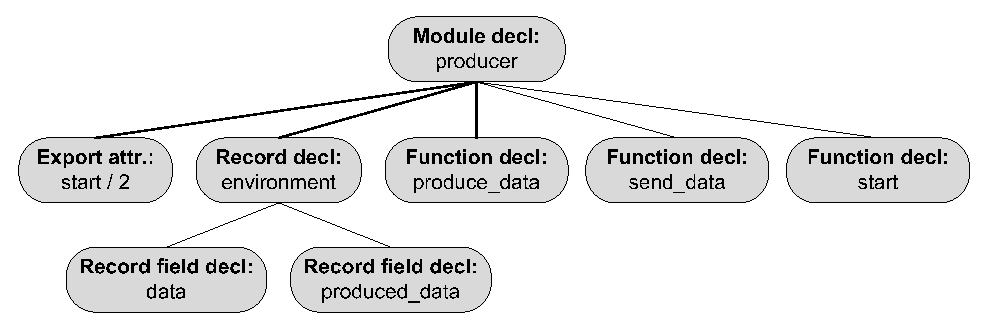
\includegraphics[width=\textwidth]{translation/ast_to_est/graphics/producerest01.eps}
\caption{The producer module of the EST}
\label{fig:prodmoduledecl}
\end{figure}

To give an impression of the translation from an AST to an EST we take a look at the producer-consumer system. Figure \ref{fig:prodmoduledecl} shows how a part of the producer is represented in the generated EST. In the following we explain how this EST and some of its subtrees are created.

\subsection{Performing the Translation}
In this section we first describe how AST processes are translated into EST module declarations. Next, we describe how global variables are translated into modules which can be used to share data among processes. Then we explain how AST blocks are translated into functions, and how a \code{start} function is created in each module. At the end of this section we describe a special system module responsible for spawning process instances.

\subsubsection{Process Nodes in the AST}
For each AST process node we create an EST \emph{module declaration}. Figure \ref{fig:prodmoduledecl} shows the \code{producer} module declaration for the producer-consumer system. AST processes contain process variables which are shared among blocks in that specific process. This kind of variables are not directly supported in Erlang, but by having a dedicated \emph{environment} record which is carried along in the function calls we get the same result as with process variables. For each AST process variable a field with the same name is created in the environment record. In Fig. \ref{fig:prodmoduledecl} we see the record declaration \code{environment}. There are two process variables \code{produced\_data} and \code{data} in the AST, thus the environment contains two \emph{record field declarations} corresponding to \code{produced\_data} and \code{data}.

\subsubsection{Global Variable Declarations}
Global variables in the AST are used to share data between processes. There is no native equivalent to global variables in the Erlang language, but instead we have constructed a module which can be used to spawn processes that acts like global variables. The module we create is identical to the module \code{shared} described in section \ref{subsec:thesharedstore}.

\subsubsection{Block Nodes in the AST}
An AST process contains a number of blocks describing the behaviour of the process. Blocks are translated into \emph{function declarations} in the EST. The \code{producer} module declaration thus contains two function declarations: \code{produce\_} \code{data} and \code{send\_data} as seen in Fig.~\ref{fig:prodmoduledecl}. Fig.~\ref{fig:prodproducefunc} shows the function declaration corresponding to the AST block \code{produce data}. As mentioned earlier the environment is given as argument to each function, thus an EST \emph{variable} \code{Env} is added to the argument list of the function declaration. 

\begin{figure}
\centering
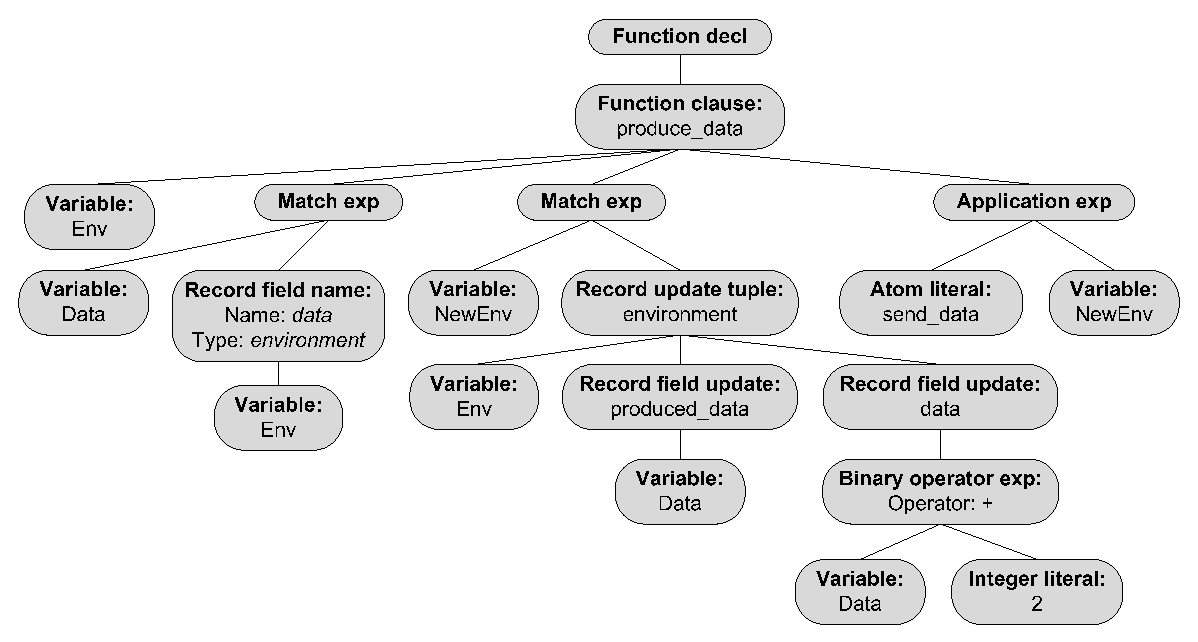
\includegraphics[width=\textwidth]{translation/ast_to_est/graphics/producerest02.eps}
\caption{The function declaration \code{produce\_data}}
\label{fig:prodproducefunc}
\end{figure}

Notice that since the EST is used by phase 5 to print the tree in a depth first traversal, the order of the EST nodes determine the semantic of the resulting Erlang program. Because, e.g., a read variable can be used to update another variable, it is important to do the reading of process variables, reading of global variables and receiving data from buffers, before writing to process variables, writing to global variables or sending data to buffers.

\paragraph*{Read process variable statements.} 
Reading a process variable is done in Erlang by accessing the corresponding field in the environment. In the EST this becomes a lookup in the record for the field with the same name as the process variable. This value is then bound to a variable which has the name given in the local variable expression of the read statement. This can be seen in Fig. \ref{fig:prodproducefunc} where the \emph{record field name expression} with the type \code{environment}, name \code{data}, and the variable \code{Env} is bound to the variable \code{Data}.

\paragraph*{Write process variable statements.}
In Erlang write statements for process variables corresponds to updating the field in the environment for that particular process variable. Fig. \ref{fig:prodproducefunc} shows how this update is represented in the EST. A \emph{record update tuple expression} containing the variable \code{Env} is bound to a variable \code{NewEnv}. The two \emph{record field update}s ensures that the fields \code{data} and \code{produced\_data} are updated corresponding to the write statements to the process variables.

\paragraph*{Receive statements.}
Receiving messages is a native construct in the Erlang language. The received messages are stored in a built-in Erlang buffer. To handle the translation of more advanced control flow constructs (presented in section~\ref{sec:advancedissues}) a buffer with extra functionality is needed. For this reason an explicit \code{buffer} process is used to receive messages. The Erlang code for the \code{buffer} module is found in appendix~\ref{appsec:buffer}. A dedicated buffer process is spawned for each receiving point of each process instance to make it equivalent to using the built-in Erlang buffers. The way to retrieve a message from the buffer is to send the atom \code{get} to the buffer process and the buffer process will send the first message in the buffer back to the requesting process.

Because of the \code{buffer} process, receiving messages it translated into sending a \code{get} request followed by a \emph{receive expression}. In the consumer module we find such an EST (see Fig.~\ref{fig:receiveexp}) in the function clause \code{receive\_data}. It consist of a send expression containing the name of the buffer and the atom literal \code{get}. This is followed by a receive expression with one \emph{receive clause} with the pattern consisting of a variable \code{Data}. The clause body contains one expression, namely the variable \code{Data}. This makes the variable (containing the received data) the return value of the receive expression and thus available in the remaining part of the function.

\begin{figure}[h!]
\centering
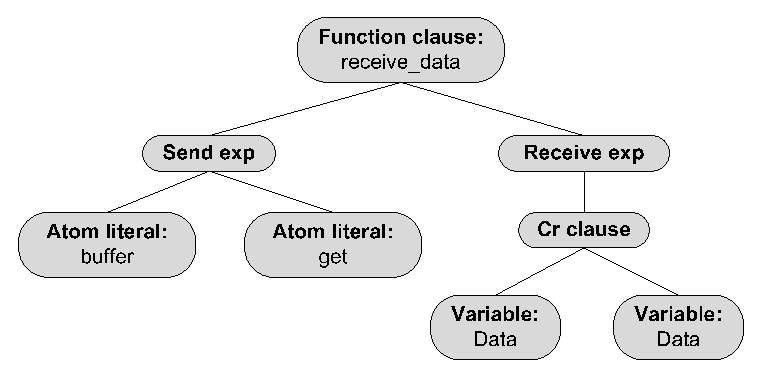
\includegraphics[scale=0.7]{translation/ast_to_est/graphics/producerest03.eps}
\caption{The receive expression subtree of the EST}
\label{fig:receiveexp}
\end{figure}

\paragraph*{Send statements.}
Since message passing is native in the Erlang language this is simply translated into a send expression in the EST. The recipient of the message is given by a buffer and an expression identifying the receiving process. In a send expression the identifier expression evaluates to an integer and together with the buffer it is possible to address the receiver of the message. The send expression furthermore contains an atom literal \code{send} indicating that the message should be added to the buffer. 

\paragraph*{Read global variable statements.}
As explained in section \ref{sec:producerconsumererlang} we have translated global variables into a shared process used to exchange data. Thus reading a global variable is translated to first sending a \code{\{get, id\}} request to the shared process corresponding to the global variable and then receiving some data from the shared process. In Fig. \ref{fig:readglobalvarexp} we see how this works in the \code{send\_data} function of the \code{producer} module. In the EST there is a \emph{send expression} containing the receiver \code{next\_consumer} and a \emph{tuple} containing the atom literal \code{get} and the application expression \code{self()}. An \emph{application expression} is a function call and the Erlang built-in function \code{self()} returns the process ID of the calling process. The send expression is then followed by a receive expression ready to receive the data from the shared process.

\begin{figure}[h!]
\centering
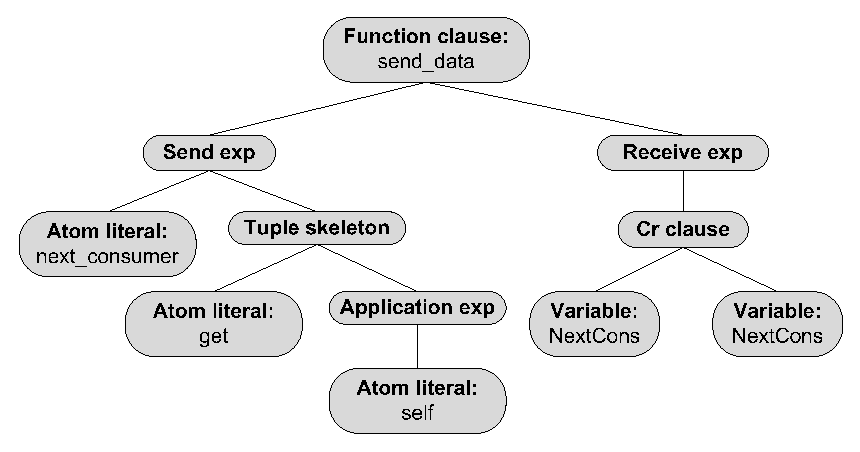
\includegraphics[scale=0.7]{translation/ast_to_est/graphics/producerest04.eps}
\caption{The subtree of the EST reading a global variable}
\label{fig:readglobalvarexp}
\end{figure}

\paragraph*{Write global variable statements.}
In the EST, write statements to global variables are translated into \emph{send expressions} which sends the value to be written to the shared process. The function \code{send\_data} contains a send expression which is a translation of the write statement to the global variable \code{NextConsumer}. This is done by sending a \emph{tuple} containing the atom literal \code{set} and the expression \code{nextcons}.

\paragraph*{Goto statements.}
\emph{Goto} statements in the AST are divided into \emph{unconditional} and \emph{conditional}. Unconditional goto statements are simply translated into application expressions in the EST. In the EST for the function \code{produce\_data} (see Fig.~\ref{fig:prodproducefunc}) we see the application expression containing the atom literal \code{send\_data} and the argument \code{NewEnv}. Conditional goto statements are explained in section \ref{sec:advancedissues}. 


\subsubsection{The Start Function}
The purpose of the \code{start} function is to initialise the environment in the process and call the first function to be executed. The start function takes a number of arguments used to initialise the environment. For each AST process variable an EST variable with the same name as the process variable is added to the function clause argument list. This can be seen in Fig.~\ref{fig:startfunction} showing the \code{start} function in the module \code{producer}. The function clause contains a variable \code{Produced\_data} and a variable \code{Data} as arguments corresponding to the process variable of the same names.  

\begin{figure}[h]
\centering
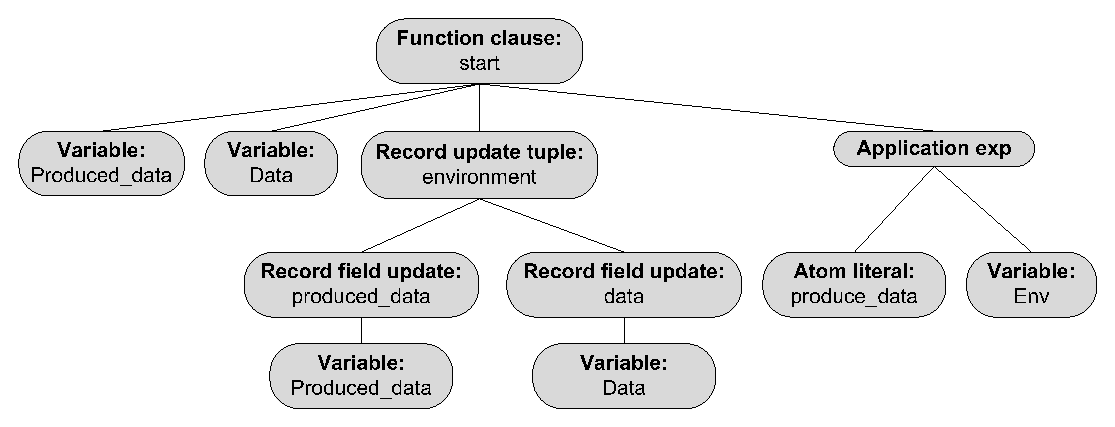
\includegraphics[width=\textwidth]{translation/ast_to_est/graphics/producerest05.eps}
\caption{The subtree of the EST showing the \code{start} function clause}
\label{fig:startfunction}
\end{figure}

The environment is then initialised by creating an environment record where the arguments are used to update to corresponding field. This record is then bound to the variable \code{Env}. In Fig.~\ref{fig:startfunction} this is seen in the match expression where a record update tuple expression is matched to the variable \code{Env}. The record update tuple expression contains two record field update expression: one assigning the variable \code{Produced\_data} to the field \code{produced\_data}, and one assigning the variable \code{Data} to the field \code{data}.

In an AST process there is a entry block which contains a goto statement to the first block to be called. In the EST, an application expression is created calling the function corresponding to the first block. In the \code{producer} module the start function shown in Fig.~\ref{fig:startfunction} calls the function \code{produced\_data}.

The \code{start} function is exported in the module such that it can be called from outside. This can be seen in Fig. \ref{fig:prodmoduledecl} where an \emph{export attribute} exports the \code{start} function taking two arguments.

\subsubsection{Spawning the Process Instances}
We have chosen to have a dedicated module which spawns a process for each process instance. It also spawns the \code{buffer} processes and a \code{shared} process for each global variable. In Fig.~\ref{fig:systemmoduledecl}, the \code{start} function clause of the \code{system} module for the producer-consumer system is shown. It is responsible for spawning process instances, thus in the producer-consumer system this becomes: two producers, two consumers and two buffers belonging to those consumers, and a shared instance. In the \code{start} function clause we find an application expression calling the Erlang built-in function \emph{register} given a name and an application expression calling the Erlang built-in function \emph{spawn}.

\begin{figure}[h]
\centering
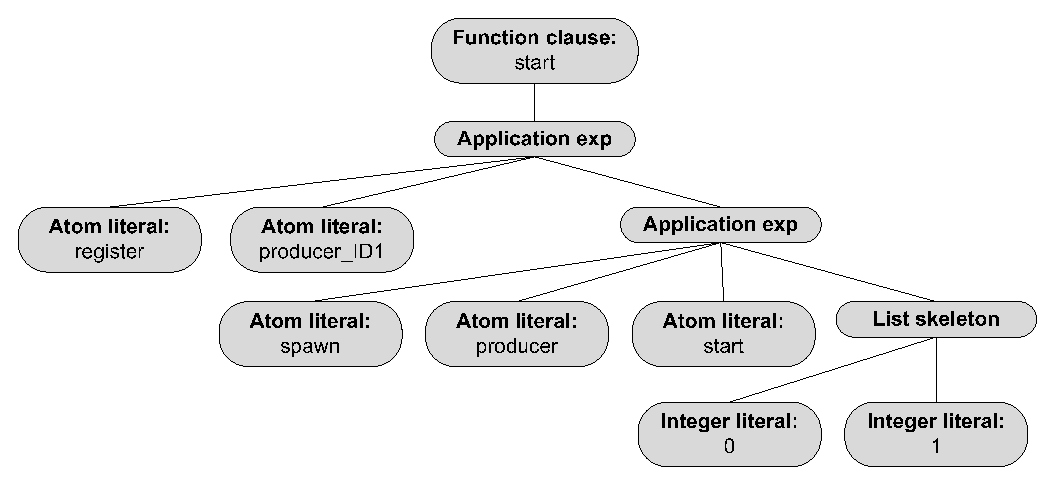
\includegraphics[width=\textwidth]{translation/ast_to_est/graphics/producerest06.eps}
\caption{The function clause \code{start} of the \code{system} module}
\label{fig:systemmoduledecl}
\end{figure}

\subsection{The Structure of the EST}
We describe the EST using EBNF and part of it is shown in Fig.~\ref{fig:ESTEBNF} (the full version can be found in appendix \ref{app:estebnffull}). The EST EBNF is based on the Erlang language specification grammar \cite{RefWorks:91}. The first definition is a \code{Program} which consists of zero or more \code{ModuleDecl}s. A \code{ModuleDecl} has a name, zero or more \code{HeaderForm}s and a \code{ProgramForm}. A \code{HeaderForm} is used to export functions and declare records. A \code{FunctionDecl} consist of a number of \code{FunctionClause}s which contains a function symbol, zero or one \code{pattern} (the arguments to the function clause) and zero or more \code{expression}s (the body of the function clause). A \code{Pattern} is, e.g., an atom literal, or a variable. An \code{Expression} is can be a \code{ApplicationExp}, \code{AtomicLiteral}, \code{BinaryOperatorExp}, \code{MatchExp}, \code{ReceiveExp}, \code{RecordExp}, \code{SendExp}, or a \code{Variable}. An \code{ApplicationExp} contains an expression (which could be an \code{AtomLiteral}) specifying which function to call, and a list of expressions which is the arguments to the function call.
\begin{figure}
\footnotesize
\begin{verbatim}
<Program>              ::= *<ModuleDecl>
<ModuleDecl>           ::= <ModuleName> *<HeaderForm> <ProgramForm> 
<ModuleName>           ::= string
<HeaderForm>           ::= <ExportAttribute> | <RecordDecl>
<ProgramForm>          ::= <FunctionDecl> | 
                           *<ProgramForm> <FunctionDecl> |
                           *<ProgramForm> <RecordDecl> 
<ExportAttribute>      ::= *<FunctionName>
<FunctionDecl>         ::= *<FunctionClause>  
<FunctionName>         ::= <FunctionSymbol> <arity>
<FunctionClause>       ::= <FunctionSymbol> ?<Pattern> *<Expression>
<Pattern>              ::= <AtomicLiteral> | <Variable>
... 
<AtomicLiteral>        ::= string
<Variable>             ::= string
<Expression>           ::= <ApplicationExp> | <AtomicLiteral> |
                           <BinaryOperatorExp> | <MatchExp> | <ReceiveExp> |
                           <RecordExp> | <SendExp> | <Variable> 
...
<ApplicationExp>       ::= <Expression> *<Expression>
<BinaryOperatorExp>    ::= <Expression> <Operator> <Expression>
<MatchExp>             ::= <Pattern> <Expression>
<ReceiveExp>           ::= *<CrClause>
<CrClause>             ::= <Pattern> *<Expression>
<RecordExp>            ::= ?<Expression> <RecordType> <RecordFieldNameExp> |
                           ?<Expression> <RecordType> <RecordUpdateTupleExp>
<RecordFieldNameExp>   ::= <RecordFieldName> 
<RecordUpdateTupleExp> ::= *<RecordFieldUpdate>
<RecordFieldUpdate>    ::= <RecordFieldName> <Expression>
<SendExp>              ::= <Expression> <Expression>
\end{verbatim}
\normalsize
\caption{The EBNF for the Erlang syntax tree}
\label{fig:ESTEBNF}
\end{figure}
